\chapter{ASP.NET MVC4}
MVC w chwili obecnej jest najnowszym frameworkiem rozwijanym przez Microsoft służącym do szybkiego tworzenia aplikacji internetowych \cite{mvc-book}. Nazwa MVC jest akronimem wzorca projektowego ,,Model View Controller'', który jest wykorzystywany do tworzenia aplikacji posiadających interfejs graficzny. Framework niejako wymusza zastosowanie go w wytwarzanej aplikacji. Wiedza na temat powyższego wzorca znacznie zwiększa jakość architektury wytwarzanej aplikacji poprzez lepszą organizację kodu.

\section{Wzorzec projektowy ,,Model View Controller''}
MVC porządkuje składowe aplikacji w trzy warstwy - warstwę modeli, widoków i kontrolerów. Każda z nich posiada swoje wyjątkowe funkcjonalności, dzięki czemu warstwy mogą być rozwijane niezależnie od siebie. Posługując się MVC sprawiamy, że nasza aplikacja staje się zgodna z jedną z głównych zasad programowania obiektowego - ,,Separation of concerns''.

\subsection{Model}
Model reprezentuje warstwę danych aplikacji. Najczęściej są to klasy, które odzwierciedlają pojęcia istotne z punktu rozwiązywanych przez program problemów. Model powinien spełniać następujące założenia:
\begin{itemize}
\item Zapewniać jednolity interfejs dostępu i zapisu danych. Dzięki temu reszta składowych aplikacji nie musi być świadoma tego w jaki sposób są one pozyskiwane.
\item Nie posiadać logiki.
\item Zmiana sposobu dostępu do danych wymagać będzie zmian jedynie w warstwie modelu.
\end{itemize}

\subsection{Widok}
Do warstwy widoku aplikacji należy każdy jej fragment, który jest widoczny dla użytkownika - składowe interfejsu graficznego. Rozwijając warstwę widoku należy pamiętać o poniższych zasadach:
\begin{itemize}
\item Widok prezentuje użytkownikowi dane w odpowiedniej oprawie graficznej.
\item Warstwa nie zna sposobu dostarczania mu udanych.
\item Widok zna strukturę dostarczanych mu danych i wie jak je interpretować.
\item Logika w widoku powinna zostać ograniczona do minimum.
\item Gdyby w przyszłości zaszła potrzeba zmiany interfejsu graficznego, zmiany dotyczyć będą jedynie warstwy widoku.
\end{itemize}

\subsection{Kontroler}
Warstwa kontrolerów zawiera logikę biznesową aplikacji. Obowiązkami Kontrolera są:
\begin{itemize}
\item Pobranie odpowiednich danych z warstwy Modelu w zależności od potrzeb użytkownika aplikacji.
\item Przygotowanie i ewentualnie wykonanie dodatkowych czynności z wykorzystaniem danych w zależności od potrzeb.
\item Spreparowanie i przekazanie danych do wybranego widoku, który zostanie wyświetlony użytkownikowi. 
\end{itemize}

\subsection{Interakcje}
Interakcje między warstwami przedstawia poniższy diagram:
\begin{figure}[h]
	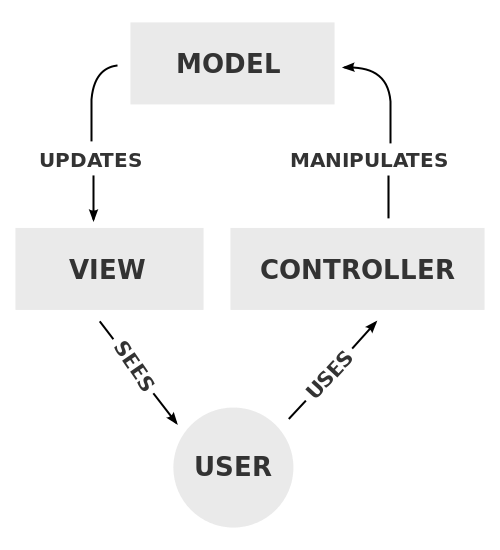
\includegraphics[height=55mm]{./img/mvc.png}
	\caption{Schemat wzorca projektowego Model View Controller}
	\label{fig:mvc-scheme}
\end{figure}


\section{Działanie frameworku}
ASP.NET MVC pozwala w łatwy oraz intuicyjny sposób obsługiwać rządania HTTP. W dużym skrócie działanie zostaje obsłużone w następujących krokach:
\begin{itemize}
\item Framework kieruje rządanie do odpowiedniego kontrolera na podstawie reguł routingu.
\item Kontroler generuje odpowiedź posługując się wybranym widokiem, do którego dostarcza spreparowane dane.
\item Dane pozyskiwane są przez klasy z warstwy modelu.
\item Silnik wypełnia widok danymi oraz zwraca odpowiedź w postaci kodu HTML.
\end{itemize}
MVC dostarcza również rozwiązań pozwalających na prosty dostęp do parametrów rządaniam, sesji, cookies oraz wiele innych. Mimo bogatej biblioteki oraz wymuszonej struktury projektu, programista posiada dużą swobodę tworząc aplikację.

\subsection{Struktura projektu}
Podczas tworzenia projektu MVC zalecane jest korzystane z domyślnej struktury projektu. W takim przypadku oprócz dobrej organizacji kodu, programista zyskuje wiele dodatkowych udogodnień takich jak uproszczone mechanizmy routingu, czy proste powiązanie kontrolera z widokiem. Nazwy folderów w intuicyjny sposób wskazują na to, co powinny zawierać. 

\begin{figure}[h]
	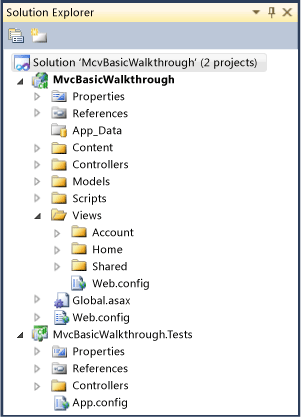
\includegraphics[height=55mm]{./img/mvc-project-structure.png}
	\caption{Struktura projektu ASP.NET MVC}
	\label{fig:mvc-project-structure}
\end{figure}

\subsection{Routing}
Najprostszym mechanizmem zarządzania routingiem w aplikacji jest trzymanie się konwencji nazewnictwa oraz umieszczania plików w odpowiednich folderach. Przykładowo url o postaci ,,http://localhost:8080/DeviceSchemes/EditScheme/20'' zostanie przekazany do kontrolera o nazwie ,,DeviceSchemesController'' i jego metody ,,EditScheme'', która powinna posiadać jeden parametr. Parametry mogą zostać rzutowane na typy proste jak i na obiekty, co znacznie upraszcza obsługę złożonych obiektów JavaScript skonwertowanych do postaci JSON. 

Drugą częścią konfigurowania routingu jest korzystanie z metod obiektu RouteCollection. Reguły definiuje się określając wzór URLa, oraz kontroler i akcję, do których rządanie zostanie skierowane. Opcjonalnie można zdefiniować też parametry rządania, które zostaną powiązane z parametrami akcji kontrolera. Aby stworzyć powiązanie z poprzedniego przykładu, należy zdefiniować trasę w następujący sposób:

\begin{lstlisting}[language=Java]
routes.MapRoute("DeviceSchemes", "DeviceSchemes/EditScheme", 
	new { controller = "DeviceScheme", action = "EditScheme", schemeId})
);
\end{lstlisting}
Obiekt RouteCollection umożliwia także tworzenie bardziej uniwersalnych tras dzięki zastosowaniu nawiasów oraz słów kluczowych w URL. Przykładowo dodanie takiego routingu:
\begin{lstlisting}[language=Java]
routes.MapRoute(
    name: "Default",
    url: "{controller}/{action}/{id}",
    defaults: new { controller = "Main", action = "Index", id = UrlParameter.Optional }
);
\end{lstlisting}
spowoduje powiązanie każdego URL do kontrolera i akcji na podstawie nazewnictwa. W przypadku gdy kontroler i akcja o odpowiednich nazwach nie zostaną znalezione, rządanie zostanie przekierowane do domyślnego kontrolera ,,MainController'' oraz akcji ,,Index'', której parametry są opcjonalne.
Podczas definiowania tras należy pamiętać, iż URL dopasowywany jest do reguł w kolejności ich definicji. Reguły należy zatem deklarować ze szczególną uwagą. Przykładowo, nie ma sensu dodawać reguł do tej samej akcji z różną liczbą parametrów w momencie gdy powyżej znajduje się deklaracja z parametrami opcjonalnymi. Należy również zwrócić uwagę na sytuację, w której powiązanie parametrów rządania z parametrami akcji jest niemożliwe. Dzieje się to, gdy typy parametrów są niezgodne i próba rzutowania kończy się wyrzuceniem wyjątku. Framework nie będzie kontynuował dopasowywania URL do kolejnych reguł.


\subsection{Warstwa kontrolerów}
Klasy będące kontrolerami powinny spełniać następujące założenia:
\begin{itemize}
\item Dziedziczyć po klasie Controller. 
\item Posiadać nazwę która kończy się słowem Controller (np. DeviceSchemesController).
\item Znajdować się w katalogu Controllers.
\end{itemize}
Wszystkie publiczne metody w kontrolerze nazywane są akcjami. W praktyce to właśnie one zawierają logikę biznesową, która obsługuje rządanie HTTP. Typ rządania z jakim powiązana zostanie akcja konfiguruje się za pomocą atrybutów (np. [HttPost] lub [HttpGet]). Rezultat działania akcji może znacznie różnić się w zależności od zwracanej przez niego wartości. Poniżej znajdują się niektóre z nich:
\begin{itemize}
\item View() - zwraca widok o nazwie odpowiadającej nazwie akcji, który musi znajdować się w katalogu o nazwie kontrolera. W przypadku kontrolera ,,DeviceSchemesController'' i akcji ,,DevicesList'' widok powinien nazywać się ,,DevicesList'' i znajdować się w katalogu o ścieżce ,,Views/DeviceSchemes''.
\item View(,,nazwa widoku'') - działa jak wyżej z tą różnicą, iż zamiast nazwy domyślnej można podać jako parametr.
\item View(obiekt modelu) - tworzy tak zwany ,,typowany widok''. Szczegóły na jego temat znajdują się w następnym podrozdziale.
\item Redirect(,,url'') - przekierowuje na podany w parametrze adres.
\item RedirectToAction(,,nazwa akcji'', ,,nazwa kontrolera'', [opcjonalne parametry]) - pozwala przekierować rządanie do kolejnej akcji.
\item Json(obiekt) - konwertuje dany obiekt do postaci Json. Pozwala to na wygodną obsługę rządań asynchronicznych.
\end{itemize}
Wszystkie powyższe metody pomocnicze znajdują się w klasie Controller. Dzięki tej klasie możliwe jest również łatwe przesyłanie dowlonych obiektów do zwracanego z kontrolera widoku. Służą do tego obiekty ViewBag i ViewData. ViewData jest mapą, z której można korzystać w następujący sposób:
\begin{lstlisting}[language=Java]
ViewData["lastProjectId"] = lastProjectId;
int lastId = (int) ViewData["lastProjectId"];
\end{lstlisting}
Minusem mapy ViewData jest to, iż wszystkie wpisywane do niej obiekty są typu Object.
Inaczej jest w przypadku ViewBag, który jest dynamicznie tworzonym obiektem.  Obiekt ten utrzymuje typy przechowywanych danych, a korzystanie z niego wygląda następująco:
\begin{lstlisting}[language=Java]
ViewData.lastProjectId = lastProjectId;
int lastId = ViewData.lastProjectId;
\end{lstlisting}

\subsection{Przykładowy kontroler}
Poniżej znajduje się fragment przykładowego kontrolera.


\begin{lstlisting}[language=Java]
namespace Elements.Controllers
{
    public class DesignerController : Controller {
    
            [HttpPost]
            public ActionResult ProjectsList()
            {
                List<Project> projectsList;
                List<DeviceScheme> schemesList;
                using (var qm = new QueryManager())
                {
                    projectsList = qm.getAllProjects();
                    schemesList = qm.GetAllDevicesSchemes();
                }
                
                ProjectsListViewModel model = new ProjectsListViewModel();
                model.DeviceSchemes = schemesList;
                model.Projects = projectsList;
    			ViewBag.model = model;
    			
                return View(model);
            }
            
            ...     
    }
}
\end{lstlisting}


\subsection{Warstwa widoków}
Widokami nazywamy pliki z kodem HTML oraz wstawkami ASPX lub Razor. Służą one do prezentowania użytkownikowi danych spreparowanych przez kontroler. Widok powinien znajdować się w katalogu Views, podkatalogu o nazwie kontrolera, a sam nosić nazwę akcji. Dzieje się tak, gdyż z reguły każdy widok związany jest z określonym kontrolerem oraz akcją. 
Wstawki ASPX oraz Razor służą do dodawania dynamicznie wygenerowanej treści do widoków. Dzięki nim możliwe jest uzyskanie dostępu do klas pomocniczych oraz obiektów modeli (ViewBag, ViewData, Model) i sesji (Session). W powyższych wstawkach możliwe jest również korzystanie z kodu C\#, co umożliwia widokom posiadać logikę. Należy jednak pamiętać, że kod w widokach powinien służyć jedynie do prezentacji danych, a nie zastępować logiki biznesowej kontrolerów. Warto zauważyć, że kod zawarty we wstawkach wykonywany jest po stronie serwera w trakcie renderowania widoku. Do wykonywania działań w aplikacji po stronie klienta używana jest technologia JavaScript. Przykładowy fragment widoku z wykorzystaniem wstawek Razor wygląda następująco:

\begin{lstlisting}[language=HTML]
<div id="projectsContainer" class="boxContainer">
    <div class="header">
        <h1>Lista wizualizacji</h1>
    </div>
    <div class="content gradiendBackgroundGray">
        <div id="addProject" class="box addBox"><span>+</span></div>

        @foreach (var project in Model.Projects)
        {
            <div class="box projectBox boxGradientBackground" data-projectname="@project.Name" data-projectid="@project.Id">
                <button class="btn btn-danger actionButton removeButton"><span class="glyphicon glyphicon-remove"></span></button>
                <button class="btn btn-success actionButton updateButton"><span class="glyphicon glyphicon-pencil"></span></button>
                <h4 class="name">@project.Name</h4>
                <p><span class="bold">Grupa: </span><span class="deviceSchemeName">@project.DeviceScheme.Name</span></p>
                <p><span class="bold">Opis: </span><span class="description">@project.Description</span></p>
                <button class="btn btn-primary actionButtonBig viewProjectButton"><span class=" glyphicon glyphicon-search"></span></button>
            </div>
        }
    </div>
</div>
\end{lstlisting}

\subsection{Cykl życia aplikacji}
Rozdział ten zawiera krótki opis życia aplikacji ASP.NET MVC oraz jej składowych. Z punktu widzenia programisty są to bardzo istotne informacje, gdyż tworzenie obiektów klas definiowanych przez programistę często wykonywane jest przez framework. Aby mieć pełną kontrolę nad towrzoną aplikacją warto jest znać kolejne kroki podejmowane przez MVC podczas obsługi rządania HTTP.

W momencie gdy aplikacja jest uruchamiana na serwerze wywoływane są metody klasy MvcApplication, których zadaniem jest konfiguracja aplikacji. Klasa ta jest umieszczona w pliku Global.asax.cs. Pierwszą wywoływaną metodą klasy jest Application\_Start. Znajduje się w niej między innymi wywołanie wcześniej wspomnianej metody RegisterRoutes, w której definiuje się trasy routingu. W klasie MvcApplication można dodatkowo zdefiniować ,,listenery'' - metody, które zostają wywołane przez framework w momencie różnych zdarzeń podczas życia aplikacji. Mogą to być na przykład zdarzenia tworzenia oraz niszczenia sesji.
Od momentu odebrania rządania HTTP do zwrócenia użytkownikowi odpowiedzi framework wykonuje następujące czynności:
\begin{itemize}
\item URL zapytania zostaje porównane z definicjami tras.
\item W momencie, gdy zapytanie zostanie dopasowane do kontrolera i akcji framewrok tworzy obiekt odpowiedniej klasy kontrolera. 
\item Wywoływana jest odpowiednia akcja kontrolera. Gdy posiada ona parametry, są one przekazywane do akcji. Parametry są rzutowane na odpowiednie typy jeśli zachodzi taka potrzeba. W przypadku niepowodzenia rzutowania zostanie wyrzucony wyjątek.
\item W zależności od typu zwracanej wartości przez akcję, użytkownikowi użytkownikowi zwracana jest odpowiedź. Może to byc kod HTML, obiekt JSON lub pojedyncza wartość.
\end{itemize}


Mechanizm obsługi rządania przedstawia poniższy diagram:
\begin{figure}[h]
	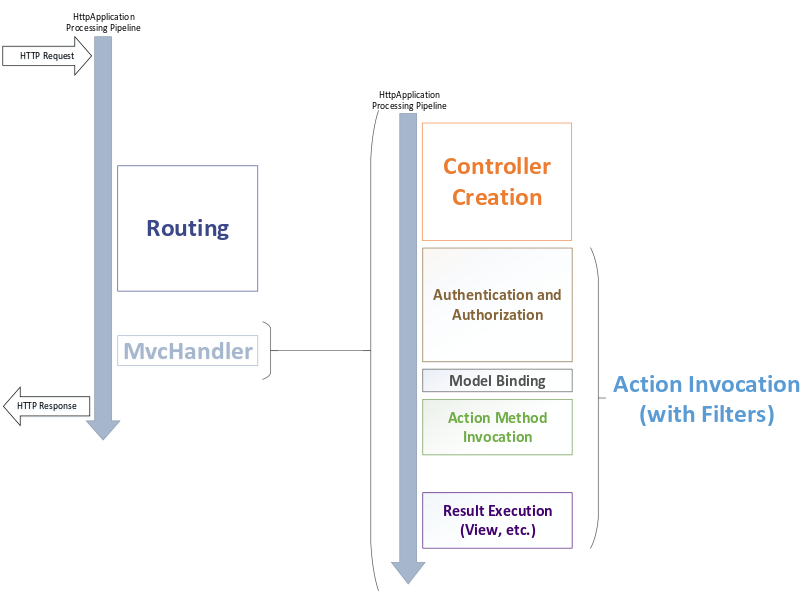
\includegraphics[width=140mm]{./img/mvc-diagram.png}
	\caption{Obsługa rządania HTTP}
	\label{fig:mvc-diagram}
\end{figure}


\subsection{Warstwa modeli}
Warstwa modeli zawiera wszystkie klasy, które opisują elementy składowe rozwiązywanego problemu. Warstwa ta powinna zawierać również mechanizmy pobierania oraz zapisu danych modeli. 
Framework pozostawia w tym miejscu programiście dużą swobodę działania. Nie ma narzuconej metody implementacji warstwy modeli. Jest to logiczne, gdyż aplikacja może pobierać i zapisywać dane na wiele sposobów, na przykład poprzez bazę danych, kolejki, pliki, itp. 
Przykładowa klasa należąca do warstwy może wyglądać następująco:
\begin{lstlisting}[language=Java]
public class DeviceScheme
{
        public int Id { get; set; }
        public string Name { get; set; }
        public string DevicesNames { get; set; }
        public IList<Project> Projects { get; set; }
}
\end{lstlisting}
Łatwo zauważyć, iż nie posiada ona żadnej logiki, jedynie istotne atrybuty, które ją opisują.